\documentclass[conference]{IEEEtran}

\usepackage{cite}
\usepackage{amsmath,amssymb,amsfonts}
\usepackage{algorithm}
\usepackage{algpseudocode}
\usepackage{fontspec}
\usepackage{fancyhdr}
\usepackage{graphicx}
\usepackage{booktabs}
\usepackage{array}
\usepackage{textcomp}
\usepackage{xcolor}
\usepackage{url}
\usepackage{xurl}
\usepackage{lettrine}
\usepackage{float}
\usepackage{placeins}
\usepackage{multirow}
\usepackage[hidelinks,breaklinks=true]{hyperref}

\def\BibTeX{{\rm B\kern-.05em{\sc i\kern-.025em b}\kern-.08em
    T\kern-.1667em\lower.7ex\hbox{E}\kern-.125emX}}

\IfFontExistsTF{Times New Roman}
  {\setmainfont{Times New Roman}}
  {\setmainfont{TeX Gyre Termes}}

\renewcommand{\LettrineFontHook}{}
\raggedbottom

\pagestyle{fancy}
\fancyhf{}
\renewcommand{\headrulewidth}{0pt}
\renewcommand{\footrulewidth}{0pt}
\fancyfoot[C]{{\footnotesize Makalah II4021 Kriptografi, Semester II Tahun 2025/2026}}

\makeatletter
\def\section{\@startsection{section}{1}{\z@}{2.8ex plus 1.8ex minus 0.6ex}%
{1.3ex plus 1ex minus 0ex}{\normalfont\normalsize\centering\scshape}}%
\def\subsection{\@startsection{subsection}{2}{\z@}{2.1ex plus 1.5ex minus 0.5ex}%
{1.0ex plus .5ex minus 0ex}{\normalfont\normalsize\itshape}}%
\def\subsubsection{\@startsection{subsubsection}{3}{\parindent}{0ex plus 0.1ex minus 0.1ex}%
{0ex}{\normalfont\normalsize\itshape}}%
\makeatother

\newcommand{\ulineurl}[1]{\url{#1}}
\newcommand{\figureplaceholder}[3]{%
\fbox{\parbox[c][#2][c]{#1}{\centering\textbf{#3}\\[0.35em]\footnotesize Placeholder to be replaced by the rendered asset from the \texttt{images/} directory.}}}
\urlstyle{same}

\begin{document}
\bstctlcite{PQCBSTControl}

\title{A Comparative Study of ML-DSA and SLH-DSA\\
for Post-Quantum Firmware Signing\\
in Secure Firmware Updates}

\author{\IEEEauthorblockN{Nayaka Ghana Subrata -- 13523090\textsuperscript{1,2}}
\IEEEauthorblockA{\textit{Department of Informatics Engineering} \\
\textit{School of Electrical Engineering and Informatics} \\
\textit{Institut Teknologi Bandung, Jl. Ganesha 10, Bandung 40132, Indonesia} \\
{\normalfont \textsuperscript{1}\underline{13523090@std.stei.itb.ac.id}, \textsuperscript{2}\underline{nayakaghana39@gmail.com}}}
}

\maketitle
\thispagestyle{empty}
\vspace{0.5em}

\begin{abstract}
\textbf{Firmware signatures anchor secure boot and firmware update trust, yet many deployed systems still rely on RSA or ECDSA, both of which are vulnerable to sufficiently large quantum computers. Replacing a classical signature with a post-quantum algorithm is not enough on its own because firmware deployment also depends on anti-rollback controls, device binding, immutable boot ROM constraints, and migration policies that determine which signatures are acceptable over time. This paper evaluates the suitability of ML-DSA and SLH-DSA for post-quantum firmware signing by combining standards-based parameter analysis with a modular Python prototype that models package metadata, migration policies, and firmware-size-dependent overhead while also executing real PQC signing and verification through local Python bindings. The study compares classical baselines, post-quantum signatures, and dual-signature migration strategies across four firmware sizes from 64 KB to 4 MB. It also simulates classical-only, PQC-only, either-valid, both-required, and version-gated verification policies. The results show that ML-DSA provides the most practical general-purpose path for firmware signing because its signatures are much smaller than those of SLH-DSA while remaining post-quantum secure. SLH-DSA remains valuable as a conservative backup because its security depends only on hash-function assumptions, but its large signatures can impose double-digit percentage overhead on small boot components. The policy analysis further shows that unrestricted either-valid migration can preserve a downgrade path to classical signatures, whereas authenticated version-gated policies and both-required policies prevent that class of failure.}
\end{abstract}

\begin{IEEEkeywords}
post-quantum cryptography, firmware signing, secure boot, ML-DSA, SLH-DSA, downgrade resistance, anti-rollback, algorithm agility
\end{IEEEkeywords}

\section{Introduction}

\lettrine[lines=3,lhang=0.08,loversize=0.15,findent=0.5em,nindent=0em]{F}{irmware} update mechanisms are one of the most security-critical components of modern embedded systems. Routers, secure elements, industrial controllers, vehicles, and consumer IoT devices all rely on firmware to initialize hardware and enforce privileged security decisions. If an attacker can install unauthorized firmware, the entire higher-level security architecture can be bypassed. For that reason, secure boot and update systems typically require a digital signature before code is executed or accepted for installation.

This trust model is under long-term pressure from quantum computing. NIST finalized the first post-quantum cryptography standards on August 13, 2024, including FIPS 204 for ML-DSA and FIPS 205 for SLH-DSA, and encouraged organizations to begin migrating to the new standards as soon as possible \cite{nist_pqc_release,fips204,fips205}. The migration question is especially urgent for firmware because hardware development and deployment cycles are long. As observed in the OpenTitan secure-boot context, a boot ROM designed today may remain fielded for ten to twenty years, and some early verification code can never be changed after manufacture \cite{opentitan_secure_boot,zerorisc_opentitan}.

However, firmware signing is not merely a benchmark problem about key size and verification time. A realistic update system must also authenticate metadata, prevent rollback to older vulnerable images, bind images to the intended device class, and avoid migration policies that allow attackers to force a fallback to weaker signatures. A package that carries a valid post-quantum signature but leaves the algorithm identifier or minimum bootloader version unsigned can still fail to provide an adequate security boundary.

This paper therefore studies post-quantum firmware signing as a systems problem rather than as a narrow primitive replacement. The focus is on ML-DSA and SLH-DSA because NIST positions ML-DSA as the primary digital signature standard and SLH-DSA as a backup based on a different mathematical approach \cite{nist_pqc_release}. The same migration pressure is visible in industry firmware guidance such as the UEFI Forum's post-quantum update whitepaper \cite{uefi_pqc_whitepaper}. Classical baselines, especially RSA-PSS and ECDSA P-256, are included because they remain dominant in legacy firmware ecosystems and define the practical migration target.

The main contributions of this work are as follows:
\begin{enumerate}
\item A firmware-oriented comparative analysis of RSA-PSS, ECDSA P-256, ML-DSA, and SLH-DSA that emphasizes signature size, key size, conservative security assumptions, and bootloader suitability rather than raw cryptographic novelty.
\item A proposed PQC-ready firmware package design that signs both metadata and firmware content, supports anti-rollback and algorithm agility, and explicitly binds accepted signature algorithms into authenticated policy state.
\item A modular Python prototype that models firmware package metadata and migration policies, generates reproducible evaluation tables, and performs real ML-DSA and SPHINCS+-family signing and verification through local PQC bindings.
\item An evaluation that quantifies signature overhead for firmware images from 64 KB to 4 MB and simulates how five migration policies handle downgrade, rollback, and tampering cases.
\end{enumerate}

The remainder of the paper is organized as follows. Section II reviews firmware update, secure boot, and the relevant signature families. Section III defines the threat model and security requirements. Section IV compares classical and post-quantum signature options. Section V proposes the firmware package structure and verification logic. Section VI describes the modular prototype. Section VII presents the evaluation results. Section VIII discusses deployment trade-offs, and Section IX concludes the paper.

\section{Background}

\subsection{Firmware Update and Secure Boot}

Firmware update is the process of replacing low-level device software after deployment. Unlike ordinary application updates, a firmware update often changes the software that initializes memory protection, configures device identity, and launches later execution stages. Consequently, a malicious firmware image can compromise the entire platform.

Secure boot addresses this risk by verifying each stage before handing control to the next stage. A root of trust verifies the first mutable component, which then verifies the following stage, and so on. OpenTitan documents this model explicitly: the immutable ROM authenticates the next image, enforces execution permissions, and fails closed if signature verification does not succeed \cite{opentitan_secure_boot}. Firmware signing therefore must be understood as a chain-of-trust mechanism rather than a single isolated signature check.

\begin{figure*}[!t]
\centering
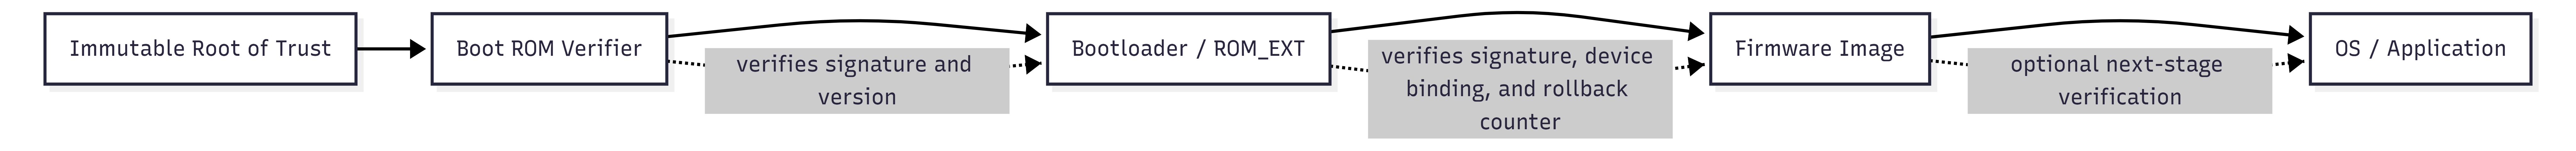
\includegraphics[width=0.94\textwidth]{../images/boot.png}
\caption{Secure-boot chain from immutable root of trust to firmware and later execution stages.}
\label{fig:secureboot}
\end{figure*}

\subsection{Classical and Post-Quantum Digital Signatures}

Firmware signing today is dominated by classical public-key signatures such as RSA-PSS and ECDSA. FIPS 186-5 specifies ECDSA as part of the Digital Signature Standard, while RSA-PSS remains standardized in PKCS \#1 v2.2 \cite{fips1865,rfc8017}. These schemes are mature, widely implemented, and well supported by secure boot stacks. Their long-term weakness is structural: Shor's algorithm threatens the integer-factorization and discrete-logarithm problems on which they depend.

Post-quantum signature schemes aim to remain secure even if large quantum computers become available. NIST's finalized standards provide two relevant families for this paper:
\begin{enumerate}
\item \textit{ML-DSA}, standardized in FIPS 204, is the primary NIST digital-signature standard for general use and is based on module-lattice assumptions \cite{fips204}.
\item \textit{SLH-DSA}, standardized in FIPS 205, is a stateless hash-based signature scheme that NIST positions as a backup because it relies on a different mathematical approach than ML-DSA \cite{fips205,nist_pqc_release}.
\end{enumerate}

The two schemes provide different deployment profiles. ML-DSA has larger public keys than ECDSA but much smaller signatures than SLH-DSA. SLH-DSA has very small public keys but very large signatures, trading package size for conservative hash-based assumptions.

\subsection{Authenticated Firmware Metadata}

Firmware update security depends on more than the firmware binary itself. Let $M$ denote the metadata structure and $F$ denote the firmware payload. A robust design signs a canonical digest representative such as
\begin{equation}
\mu = H(\text{Encode}(M)\ \|\ H(F)),
\label{eq:manifest_digest}
\end{equation}
where $H$ is a collision-resistant hash function and $\text{Encode}(M)$ is a deterministic serialization of device identifier, firmware version, policy version, and other control fields. Signing only the payload but leaving metadata outside the signature would let an attacker alter version counters or algorithm identifiers without invalidating the package.

\subsection{Anti-Rollback and Algorithm Agility}

A valid signature on an old image is still dangerous if that image contains a known vulnerability. Anti-rollback therefore requires a monotonic counter or trusted version store. If the device has already accepted firmware version $v_{\min}$, a new candidate with version $v$ should satisfy
\begin{equation}
v \geq v_{\min}.
\label{eq:rollback}
\end{equation}

Algorithm agility introduces a second state variable. The verifier must know not only which firmware versions are acceptable but also which signature algorithms are acceptable at a given migration stage. NIST migration guidance emphasizes that the transition to PQC is a roadmap problem rather than a single flag day \cite{nist_sp180038c,nist_ir8547}. In firmware systems this means accepted algorithms should be coupled to authenticated policy state rather than to unauthenticated update metadata.

\subsection{Related Signature Families}

Stateful hash-based schemes such as LMS and XMSS remain relevant to firmware discussions because NIST recommends them for some long-term applications in SP 800-208 \cite{sp800208}. They are not the main focus of this paper because their signing-state management introduces operational complexity. The OpenTitan experience report makes the same point in practice: stateful signatures can offer attractive size and performance properties, but mishandling signer state risks catastrophic failure \cite{zerorisc_opentitan}. For that reason, this paper concentrates on the stateless NIST PQC signatures while mentioning stateful schemes only as background.

\section{Problem Statement and Threat Model}

The main problem considered in this paper is the following: \textit{how suitable are ML-DSA and SLH-DSA for secure firmware update and secure boot systems that must survive a transition away from RSA or ECDSA?}

This question is broader than ``which signature is fastest.'' A secure answer must account for the constrained nature of bootloaders, immutable verification code, long device lifetimes, and the fact that a transition period may temporarily expose multiple signature options at once.

\subsection{Adversarial Capabilities}

The attacker is assumed to have network or supply-chain access to firmware packages in transit or at rest. In particular, the attacker may:
\begin{enumerate}
\item intercept a firmware package before installation;
\item modify the firmware payload;
\item modify metadata fields such as version counters, algorithm identifiers, or target device identifiers;
\item replay an older but once-valid package;
\item remove one signature from a dual-signed package;
\item attempt to force a migrated device to accept a classical-only signature.
\end{enumerate}

The attacker is not assumed to break the core security assumptions of ML-DSA or SLH-DSA, extract the vendor's private signing key, or rewrite immutable root-of-trust code. Those exclusions match the normal cryptographic boundary of a firmware-signing system.

\subsection{Security Requirements}

The firmware update system should satisfy the following requirements:
\begin{enumerate}
\item \textit{Authenticity:} only packages signed by the trusted vendor are accepted.
\item \textit{Integrity:} modifications to firmware or metadata are detected.
\item \textit{Device binding:} a package for one device class must not install on another device class.
\item \textit{Anti-rollback:} older vulnerable firmware must not be reinstallable.
\item \textit{Downgrade resistance:} after migration, the verifier must not be tricked into accepting weaker classical-only signatures.
\item \textit{Algorithm agility:} the accepted signature set must be updatable through authenticated policy rather than by redesigning the entire package format.
\end{enumerate}

These conditions can be expressed with a high-level acceptance predicate:
\begin{equation}
\begin{aligned}
\mathsf{Accept}(P,D) = &\ \mathsf{VerifySigSet}(P) \land \mathsf{BindDevice}(P,D) \\
&\land \mathsf{FreshVersion}(P,D) \land \mathsf{PolicyAllowed}(P,D),
\end{aligned}
\label{eq:acceptance}
\end{equation}
where $P$ is the candidate firmware package and $D$ is the verifier state of the device.

\subsection{Migration Risk}

The most subtle failure mode is policy downgrade during the transition period. Suppose a device is upgraded to a bootloader that supports both ECDSA and ML-DSA. If the policy states that \textit{either} valid signature is always sufficient, then a classical-only package remains acceptable indefinitely even after the operator intended to migrate away from classical signatures. That creates a downgrade path in which the device's long-term security is bounded by the weaker algorithm family.

By contrast, a version-gated or both-required policy can tie the accepted signature set to authenticated state. In that model, the package does not merely present a signature; it also carries the policy version and minimum bootloader version that determine how the verifier should interpret the signature set. This observation drives both the package design and the evaluation in later sections.

\section{Comparative Analysis of Signature Schemes}

\subsection{Classical Baselines}

RSA-PSS and ECDSA remain useful baselines because many firmware ecosystems already implement one of them. RSA-PSS offers conservative engineering maturity but larger signatures than ECDSA. ECDSA P-256 is especially attractive in constrained systems because it combines compact signatures with broad hardware and library support. Its main weakness for this paper is strategic rather than operational: once large-scale quantum computers are practical, the discrete-logarithm basis of ECDSA is no longer sufficient.

\subsection{ML-DSA}

ML-DSA is the natural primary post-quantum candidate because NIST standardized it specifically as the main general-purpose PQ signature standard \cite{nist_pqc_release,fips204}. Its deployment profile is attractive for firmware because its signatures are measured in a few kilobytes rather than tens of kilobytes. The trade-off is that its public keys are substantially larger than those of ECDSA, and embedded implementations may need careful optimization to control code size, stack usage, and constant-time behavior.

For firmware verification, ML-DSA's practical value is that it often shifts the cost from ``impossible to fit'' to ``engineering trade-off.'' A 2.4 KB signature is clearly larger than a 64-byte ECDSA signature, but it remains manageable inside many update packages and secure-boot manifests.

\subsection{SLH-DSA}

SLH-DSA is valuable because it is based on stateless hash-based techniques rather than lattice assumptions \cite{fips205}. That diversity matters in a migration plan: if unexpected weaknesses emerge for lattice signatures, SLH-DSA remains a NIST-standardized fallback path. The price is signature size. Even the small-signature category-1 style parameter set standardized in FIPS 205 requires a 7,856-byte signature, and higher categories grow far larger \cite{fips205}.

This footprint matters most for early boot components. If the firmware object being signed is only tens of kilobytes, then several kilobytes of signature data are no longer negligible. The OpenTitan experience report reaches a similar conclusion for secure boot: hash-based signatures can be a sensible fit when their larger signatures are still manageable for the platform, but the trade-off must be analyzed in the actual firmware context \cite{zerorisc_opentitan}.

\subsection{Hybrid and Dual Signatures}

Migration rarely happens in one step. A common transitional idea is to include both a classical and a post-quantum signature. Dual-signature packaging has two advantages. First, it allows updated verifiers to check a PQ signature while legacy verifiers continue checking a classical signature. Second, it allows phased rollout where signing infrastructure, bootloaders, and manufacturing tools do not all change at once.

The drawback is policy ambiguity. A dual-signed package is not automatically secure if the verifier is willing to accept \textit{either} signature forever. In that case, the package format carries a PQ signature, but the device remains vulnerable to classical-only fallback. The hybrid packaging strategy is therefore only as strong as the verification policy bound to it.

\begin{table*}[!t]
\caption{Representative Signature Profiles for Firmware-Signing Analysis}
\label{tab:profiles}
\centering
\scriptsize
\begin{tabular}{p{1.65in}p{0.82in}cccp{1.58in}}
\toprule
\textbf{Scheme} & \textbf{Family} & \textbf{Public Key (B)} & \textbf{Signature (B)} & \textbf{Bootloader Staging (B)} & \textbf{Practical Interpretation} \\
\midrule
RSA-PSS-2048 & Classical & 256 & 256 & 800 & Mature baseline, but not quantum-safe. \\
ECDSA P-256 & Classical & 64 & 64 & 416 & Smallest baseline signature and easy embedded fit. \\
ML-DSA-44 & Post-quantum & 1312 & 2420 & 4020 & Strong practical default for PQ migration. \\
ML-DSA-65 & Post-quantum & 1952 & 3309 & 5549 & Higher margin with moderate additional footprint. \\
ML-DSA-87 & Post-quantum & 2592 & 4627 & 7507 & Highest ML-DSA category, but noticeably heavier. \\
SLH-DSA-SHA2-128s & Post-quantum & 32 & 7856 & 8176 & Conservative backup; signature dominates package growth. \\
SLH-DSA-SHA2-192s & Post-quantum & 48 & 16224 & 16560 & Conservative but increasingly difficult for small boot stages. \\
SLH-DSA-SHA2-256s & Post-quantum & 64 & 29792 & 30144 & Very large signature footprint for constrained devices. \\
\bottomrule
\end{tabular}
\end{table*}

\subsection{Interpretation}

Table~\ref{tab:profiles} reveals the central trade-off of this paper. ML-DSA grows both public key size and signature size relative to classical signatures, but it stays within a low-kilobyte regime that is realistic for many firmware packages. SLH-DSA minimizes public-key storage yet shifts the burden into the signature itself. For a verifier that stores public keys in immutable ROM, SLH-DSA's tiny public key is attractive; for a deployment that distributes many small signed boot components, its signature size is the main obstacle.

The comparative conclusion is therefore not that one PQ scheme is globally superior. Rather, ML-DSA is the practical default for most firmware-signing deployments, while SLH-DSA is the conservative hedge that remains valuable when different security assumptions are desired strongly enough to justify its larger signatures.

\section{Proposed PQC-Ready Firmware Package Design}

The proposed package format is designed to survive algorithm migration without changing the semantic meaning of the signed data. It separates three concerns: authenticated metadata, firmware payload, and one or more signatures over a canonical manifest digest.

\begin{figure*}[!t]
\centering

\includegraphics[width=0.92\textwidth]{../images/layout.png}
\caption{Firmware package layout with authenticated metadata, firmware payload, and signature vector.}
\label{fig:pkg}
\end{figure*}

\subsection{Authenticated Fields}

The package should authenticate at least the following fields:
\begin{enumerate}
\item format version and magic bytes;
\item vendor identifier and target device identifier;
\item firmware version;
\item minimum bootloader version;
\item signature policy version;
\item accepted signature algorithm identifiers;
\item firmware size and firmware hash;
\item release timestamp or monotonic release identifier.
\end{enumerate}

These fields allow the verifier to answer the correct question: not merely ``is there a valid signature,'' but ``is there a valid signature on the correct object under the current trust policy?''

\subsection{Manifest Digest and Signature Vector}

Let $M$ denote the metadata structure and $F$ the firmware binary. The package signs the digest representative
\begin{equation}
\mu = H(\text{Encode}(M)\ \|\ H(F)).
\label{eq:signed_object}
\end{equation}
The signature vector is then defined as
\begin{equation}
\Sigma = \{(\text{alg}_{i}, \sigma_{i})\}_{i=1}^{k},
\label{eq:sig_vector}
\end{equation}
where each $\text{alg}_{i}$ is an authenticated algorithm identifier and $\sigma_{i}$ is a signature over $\mu$. This representation supports classical-only, PQC-only, and dual-signature packages without changing the manifest grammar.

\subsection{Verification Policy}

The verifier should not interpret $\Sigma$ in isolation. Instead, acceptance should be tied to a policy function that depends on bootloader state and authenticated metadata:
\begin{equation}
\mathcal{A}_{\text{req}} = \Pi(v_{\text{boot}}, v_{\text{policy}}, v_{\text{fw}}),
\label{eq:policy}
\end{equation}
where $\Pi$ maps bootloader version, policy version, and firmware version to the required signature set. This abstraction allows several concrete policies:
\begin{enumerate}
\item \textit{Classical-only}: accept only RSA or ECDSA.
\item \textit{PQC-only}: accept only ML-DSA or SLH-DSA.
\item \textit{Either-valid}: accept either classical or PQC signatures.
\item \textit{Both-required}: require both a classical and a PQ signature.
\item \textit{Version-gated}: require different signature sets before and after a migration threshold.
\end{enumerate}

Among these options, the unrestricted either-valid policy is the weakest during migration because it preserves a classical-only acceptance path indefinitely.

\begin{algorithm}[!t]
\caption{Downgrade-Resistant Firmware Verification}
\label{alg:verify}
\begin{algorithmic}[1]
\Require Device state $D$, firmware package $P=(M, F, \Sigma)$
\Ensure Accept or reject
\If{$M.\texttt{device\_id} \neq D.\texttt{device\_id}$}
    \State \Return reject
\EndIf
\If{$M.\texttt{firmware\_version} < D.\texttt{minimum\_allowed\_version}$}
    \State \Return reject
\EndIf
\If{$M.\texttt{minimum\_bootloader\_version} > D.\texttt{bootloader\_version}$}
    \State \Return reject
\EndIf
\State Compute $\mu \gets H(\text{Encode}(M)\ \|\ H(F))$
\State Determine required algorithms $\mathcal{A}_{\text{req}} \gets \Pi(D, M)$
\If{the signature set in $\Sigma$ does not satisfy $\mathcal{A}_{\text{req}}$}
    \State \Return reject
\EndIf
\ForAll{$(\text{alg}, \sigma) \in \Sigma$ required by $\mathcal{A}_{\text{req}}$}
    \If{Verify$(\text{alg}, \sigma, \mu)$ is false}
        \State \Return reject
    \EndIf
\EndFor
\State Persist the accepted firmware version
\State \Return accept
\end{algorithmic}
\end{algorithm}

\subsection{Why Metadata Must Be Signed}

The algorithm above highlights a crucial point: if the metadata used by $\Pi$ is not authenticated, then the verifier may enforce the wrong policy on otherwise valid cryptographic material. An attacker could lower the declared policy version, alter the claimed target device, or change the minimum bootloader version while leaving the payload untouched. The package format must therefore treat policy metadata as first-class signed input, not as optional transport information.

\section{Prototype Implementation}

The implementation under the \texttt{src/} directory combines package modeling, policy evaluation, and real post-quantum signature execution through local Python bindings.

\subsection{Module Structure}

The implementation is divided into the following modules:
\begin{enumerate}
\item \texttt{algorithms.py}: stores normalized algorithm profiles, including key sizes, signature sizes, and deployment notes for the classical and post-quantum schemes used in the paper.
\item \texttt{firmware\_package.py}: defines canonical metadata and firmware-package objects, including deterministic serialization for the authenticated fields.
\item \texttt{policy.py}: implements five verification policies and the device-state checks needed for downgrade and rollback analysis.
\item \texttt{pqc\_signatures.py}: provides the actual PQC backend for key generation, signing, verification, and signature attachment to firmware packages.
\item \texttt{scenarios.py}: defines representative migration scenarios such as legacy classical acceptance, post-migration PQ acceptance, classical-only downgrade attempts, metadata tampering, and rollback.
\item \texttt{evaluation.py}: computes package-overhead tables, bootloader staging footprints, and policy outcomes.
\item \texttt{generate\_tables.py}: writes the generated results as CSV files into \texttt{paper/data/} for inclusion and verification.
\item \texttt{pqc\_demo.py}: runs an end-to-end demonstration that generates ML-DSA and hash-based keys, signs a firmware package, and verifies the resulting signatures.
\end{enumerate}

\subsection{Design Choices}

The code separates cryptographic facts from policy logic. Standards-based quantities such as public-key size and signature size are stored as immutable algorithm profiles, while concrete PQC operations are isolated behind a backend wrapper.

The implementation uses the \texttt{pqcrypto} package for the concrete PQC backend. The repository-local \texttt{.deps} directory is inserted into the Python import path inside \texttt{pqc\_signatures.py}, after which the backend modules are imported explicitly. In that package, ML-DSA is exposed under the finalized names \texttt{ml\_dsa\_44}, \texttt{ml\_dsa\_65}, and \texttt{ml\_dsa\_87}. The SLH-DSA family is still exposed under the pre-standard SPHINCS+ module names, so the code maps the paper's \texttt{slh\_dsa\_*} identifiers to the corresponding SPHINCS+ SHA-2 simple variants.

The policy scenarios use deterministic firmware payload generation so that manifest hashes and measured outputs remain reproducible across runs.

\FloatBarrier
\section{Evaluation}

\subsection{Method}

The evaluation combines standards-based parameter analysis with policy simulation. Four firmware sizes are considered: 64 KB, 256 KB, 1 MB, and 4 MB. These values span the range from small boot components to ordinary field-update images. For each scheme with signature size $|\sigma|$ and firmware size $|F|$, the package overhead is
\begin{equation}
\text{Overhead}(F,\sigma) = \frac{|\sigma|}{|F|}\times 100\%.
\label{eq:overhead}
\end{equation}

The implementation also estimates the verifier's staging footprint as the sum of public-key bytes, signature bytes, authenticated metadata bytes, and a firmware digest buffer. The runtime experiment performs three trials per scheme over a 47-byte benchmark message and records mean key-generation, signing, and verification latency.

\subsection{Firmware Package Overhead}

Table~\ref{tab:overhead} and Fig.~\ref{fig:overheadplot} show the dependence of package overhead on firmware size. For a 64 KB boot component, ML-DSA-44 contributes 3.6926\% overhead, while SLH-DSA-SHA2-128s contributes 11.9873\%. At 4 MB, these values decrease to 0.0577\% and 0.1873\%, respectively.

\begin{table}[H]
\caption{Signature Overhead Across Firmware Sizes}
\label{tab:overhead}
\centering
\scriptsize
\setlength{\tabcolsep}{2.5pt}
\resizebox{\columnwidth}{!}{%
\begin{tabular}{lccccc}
\toprule
\textbf{Scheme} & \textbf{Sig. (B)} & \textbf{64 KB} & \textbf{256 KB} & \textbf{1 MB} & \textbf{4 MB} \\
\midrule
ECDSA & 64 & 0.0977\% & 0.0244\% & 0.0061\% & 0.0015\% \\
RSA-PSS & 256 & 0.3906\% & 0.0977\% & 0.0244\% & 0.0061\% \\
ML-DSA-44 & 2420 & 3.6926\% & 0.9232\% & 0.2308\% & 0.0577\% \\
ML-DSA-65 & 3309 & 5.0491\% & 1.2623\% & 0.3156\% & 0.0789\% \\
SLH-128s & 7856 & 11.9873\% & 2.9968\% & 0.7492\% & 0.1873\% \\
ECDSA+ML44 & 2484 & 3.7903\% & 0.9476\% & 0.2369\% & 0.0592\% \\
ECDSA+SLH128s & 7920 & 12.0850\% & 3.0212\% & 0.7553\% & 0.1888\% \\
\bottomrule
\end{tabular}
}
\end{table}

For large firmware images, signature size is a secondary cost. For small boot components, the gap between ML-DSA and SLH-DSA remains operationally significant.

\begin{figure}[H]
\centering
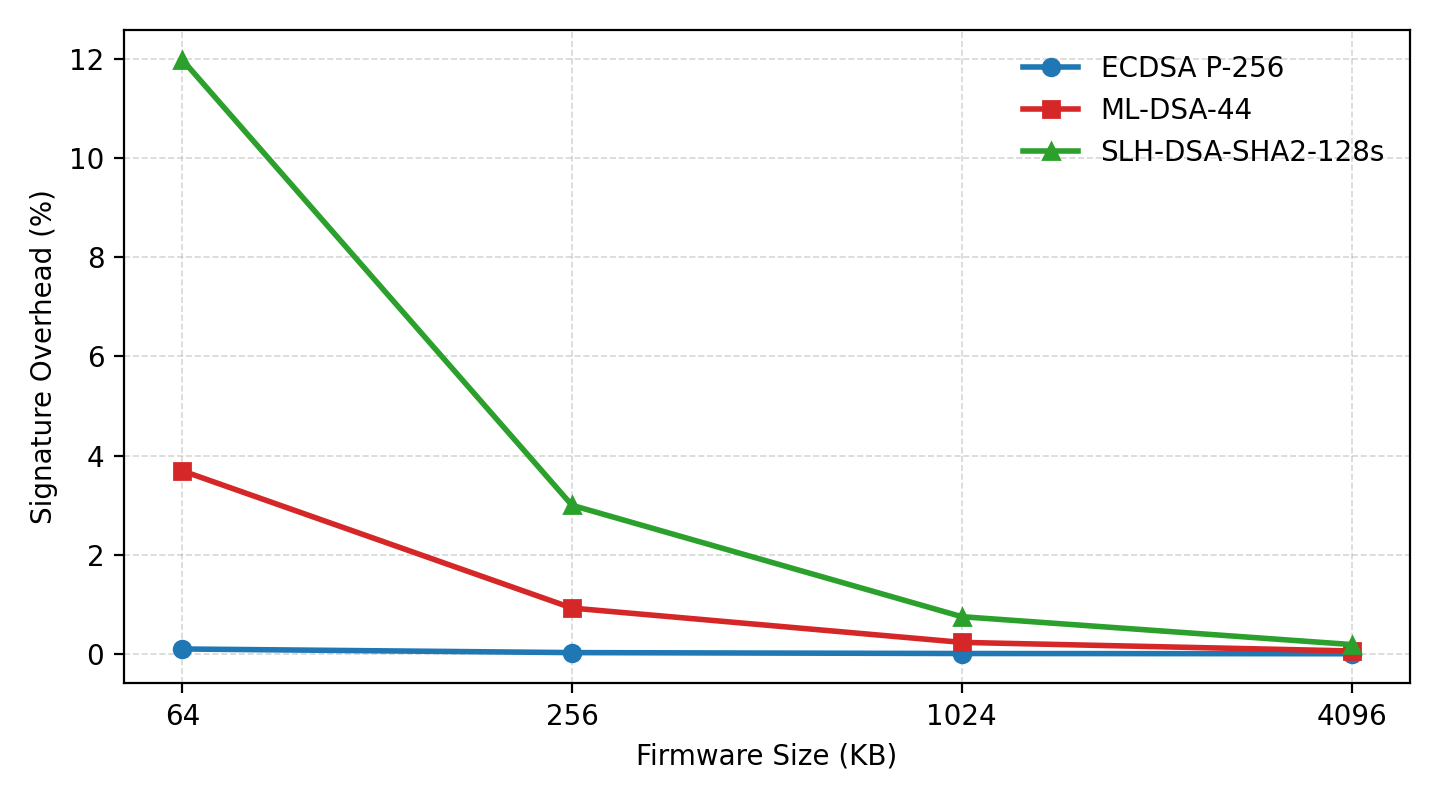
\includegraphics[width=\columnwidth]{../images/firmware_overhead_plot.png}
\caption{Measured overhead trend for representative classical and post-quantum signatures across firmware sizes.}
\label{fig:overheadplot}
\end{figure}

\subsection{Measured PQC Runtime}

Table~\ref{tab:runtime} and Fig.~\ref{fig:runtimeplot} report mean latency from the local PQC backend. ML-DSA-44 completed key generation in 0.299 ms on average, signing in 0.734 ms, and verification in 0.166 ms. In the same environment, the SLH-DSA-SHA2-128s mapping required 206.066 ms for key generation and 1430.190 ms for signing, while verification remained at 1.159 ms.

\begin{table}[H]
\caption{Measured PQC Runtime with the Local \texttt{pqcrypto} Backend}
\label{tab:runtime}
\centering
\scriptsize
\begin{tabular}{p{1.05in}cccc}
\toprule
\textbf{Scheme} & \textbf{Trials} & \textbf{KeyGen} & \textbf{Sign} & \textbf{Verify} \\
\midrule
ML-DSA-44 & 3 & 0.299 & 0.734 & 0.166 \\
SLH-DSA-SHA2-128s & 3 & 206.066 & 1430.190 & 1.159 \\
\bottomrule
\end{tabular}
\end{table}

The local benchmark indicates that ML-DSA is substantially cheaper than SLH-DSA for key generation and signing in this software setting, while both remain fast to verify relative to signing cost.

\begin{figure}[H]
\centering
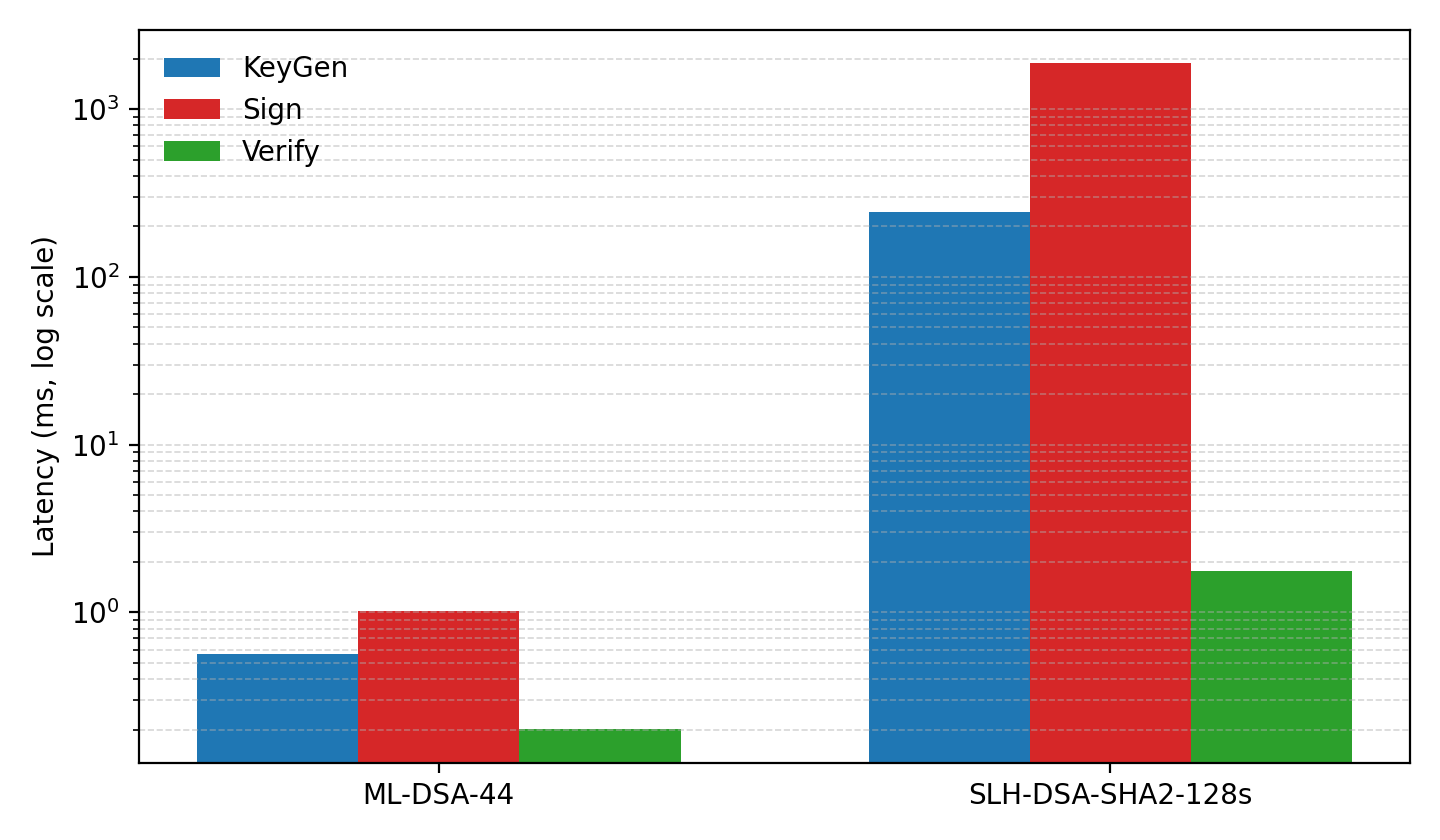
\includegraphics[width=\columnwidth]{../images/pqc_runtime_plot.png}
\caption{Measured PQC runtime. The vertical axis uses logarithmic scale.}
\label{fig:runtimeplot}
\end{figure}

\subsection{Migration Policy Simulation}

The policy simulation evaluates six scenarios across five policies. Table~\ref{tab:policy} shows that the \textit{either-valid} policy accepts a classical-only package after the migration threshold, whereas the version-gated policy rejects it.

\begin{table}[H]
\caption{Policy Simulation Outcomes (\textbf{A} = Accept, \textbf{R} = Reject)}
\label{tab:policy}
\centering
\scriptsize
\setlength{\tabcolsep}{2.5pt}
\resizebox{\columnwidth}{!}{%
\begin{tabular}{p{1.22in}ccccc}
\toprule
\textbf{Scenario} & \textbf{Cls} & \textbf{PQC} & \textbf{Either} & \textbf{Both} & \textbf{V-gated} \\
\midrule
Legacy pre-migration & A & R & A & R & A \\
PQC-only post-migration & R & A & A & R & A \\
Classical-only post-migration & A & R & A & R & R \\
Dual-signed post-migration & A & A & A & A & A \\
Tampered alg. declaration & R & R & R & R & R \\
Rollback package & R & R & R & R & R \\
\bottomrule
\end{tabular}
}
\end{table}

The both-required policy imposes the strongest migration requirement but forces every accepted post-migration package to carry both a classical and a PQ signature. The version-gated policy preserves compatibility before the threshold and removes the classical-only acceptance path after the threshold.

\subsection{Bootloader Suitability}

The bootloader staging values in Table~\ref{tab:profiles} show the same trade-off. SLH-DSA-SHA2-128s has a tiny public key but still requires 8,176 bytes of staged material in the simplified proxy model because the signature dominates. ML-DSA-44 requires 4,020 staged bytes, which is larger than classical baselines but considerably smaller than SLH-DSA.

\subsection{Summary of Findings}

The numerical results support three practical conclusions:
\begin{enumerate}
\item ML-DSA is the most balanced general-purpose PQ option for firmware signing.
\item SLH-DSA is most compelling when conservative security assumptions are worth a significant package-size penalty.
\item Downgrade resistance depends at least as much on verification policy as on the chosen signature algorithm.
\end{enumerate}

\section{Discussion}

\subsection{Why ML-DSA Is the Practical Default}

ML-DSA fits the firmware-signing use case because it offers a manageable compromise between cryptographic conservatism and deployment cost. Its signatures are much larger than ECDSA, but they remain in a range that can be tolerated by many update formats and manifests. In contrast, SLH-DSA signatures quickly become dominant on small images. If a platform must choose one PQ signature family for broad deployment today, ML-DSA is therefore the most pragmatic default.

\subsection{Why SLH-DSA Still Matters}

It would be a mistake to dismiss SLH-DSA merely because its signatures are large. NIST standardized it specifically as a backup that relies on a different mathematical basis than ML-DSA \cite{nist_pqc_release}. In high-assurance environments, that diversity is valuable. A vendor may decide to keep SLH-DSA support for recovery tooling, high-value product lines, or contingency planning even if ML-DSA is the main production choice.

\subsection{When Dual Signatures Are Justified}

Dual signatures are justified when compatibility requirements are real and temporary. They are especially useful when the installed base contains immutable verifiers that understand only classical signatures while newer devices can already verify PQ signatures. However, dual signatures should be paired with either a both-required rule or an authenticated version-gated rule. Otherwise the transition accumulates cryptographic baggage without actually removing classical exposure.

\begin{figure}[H]
\centering
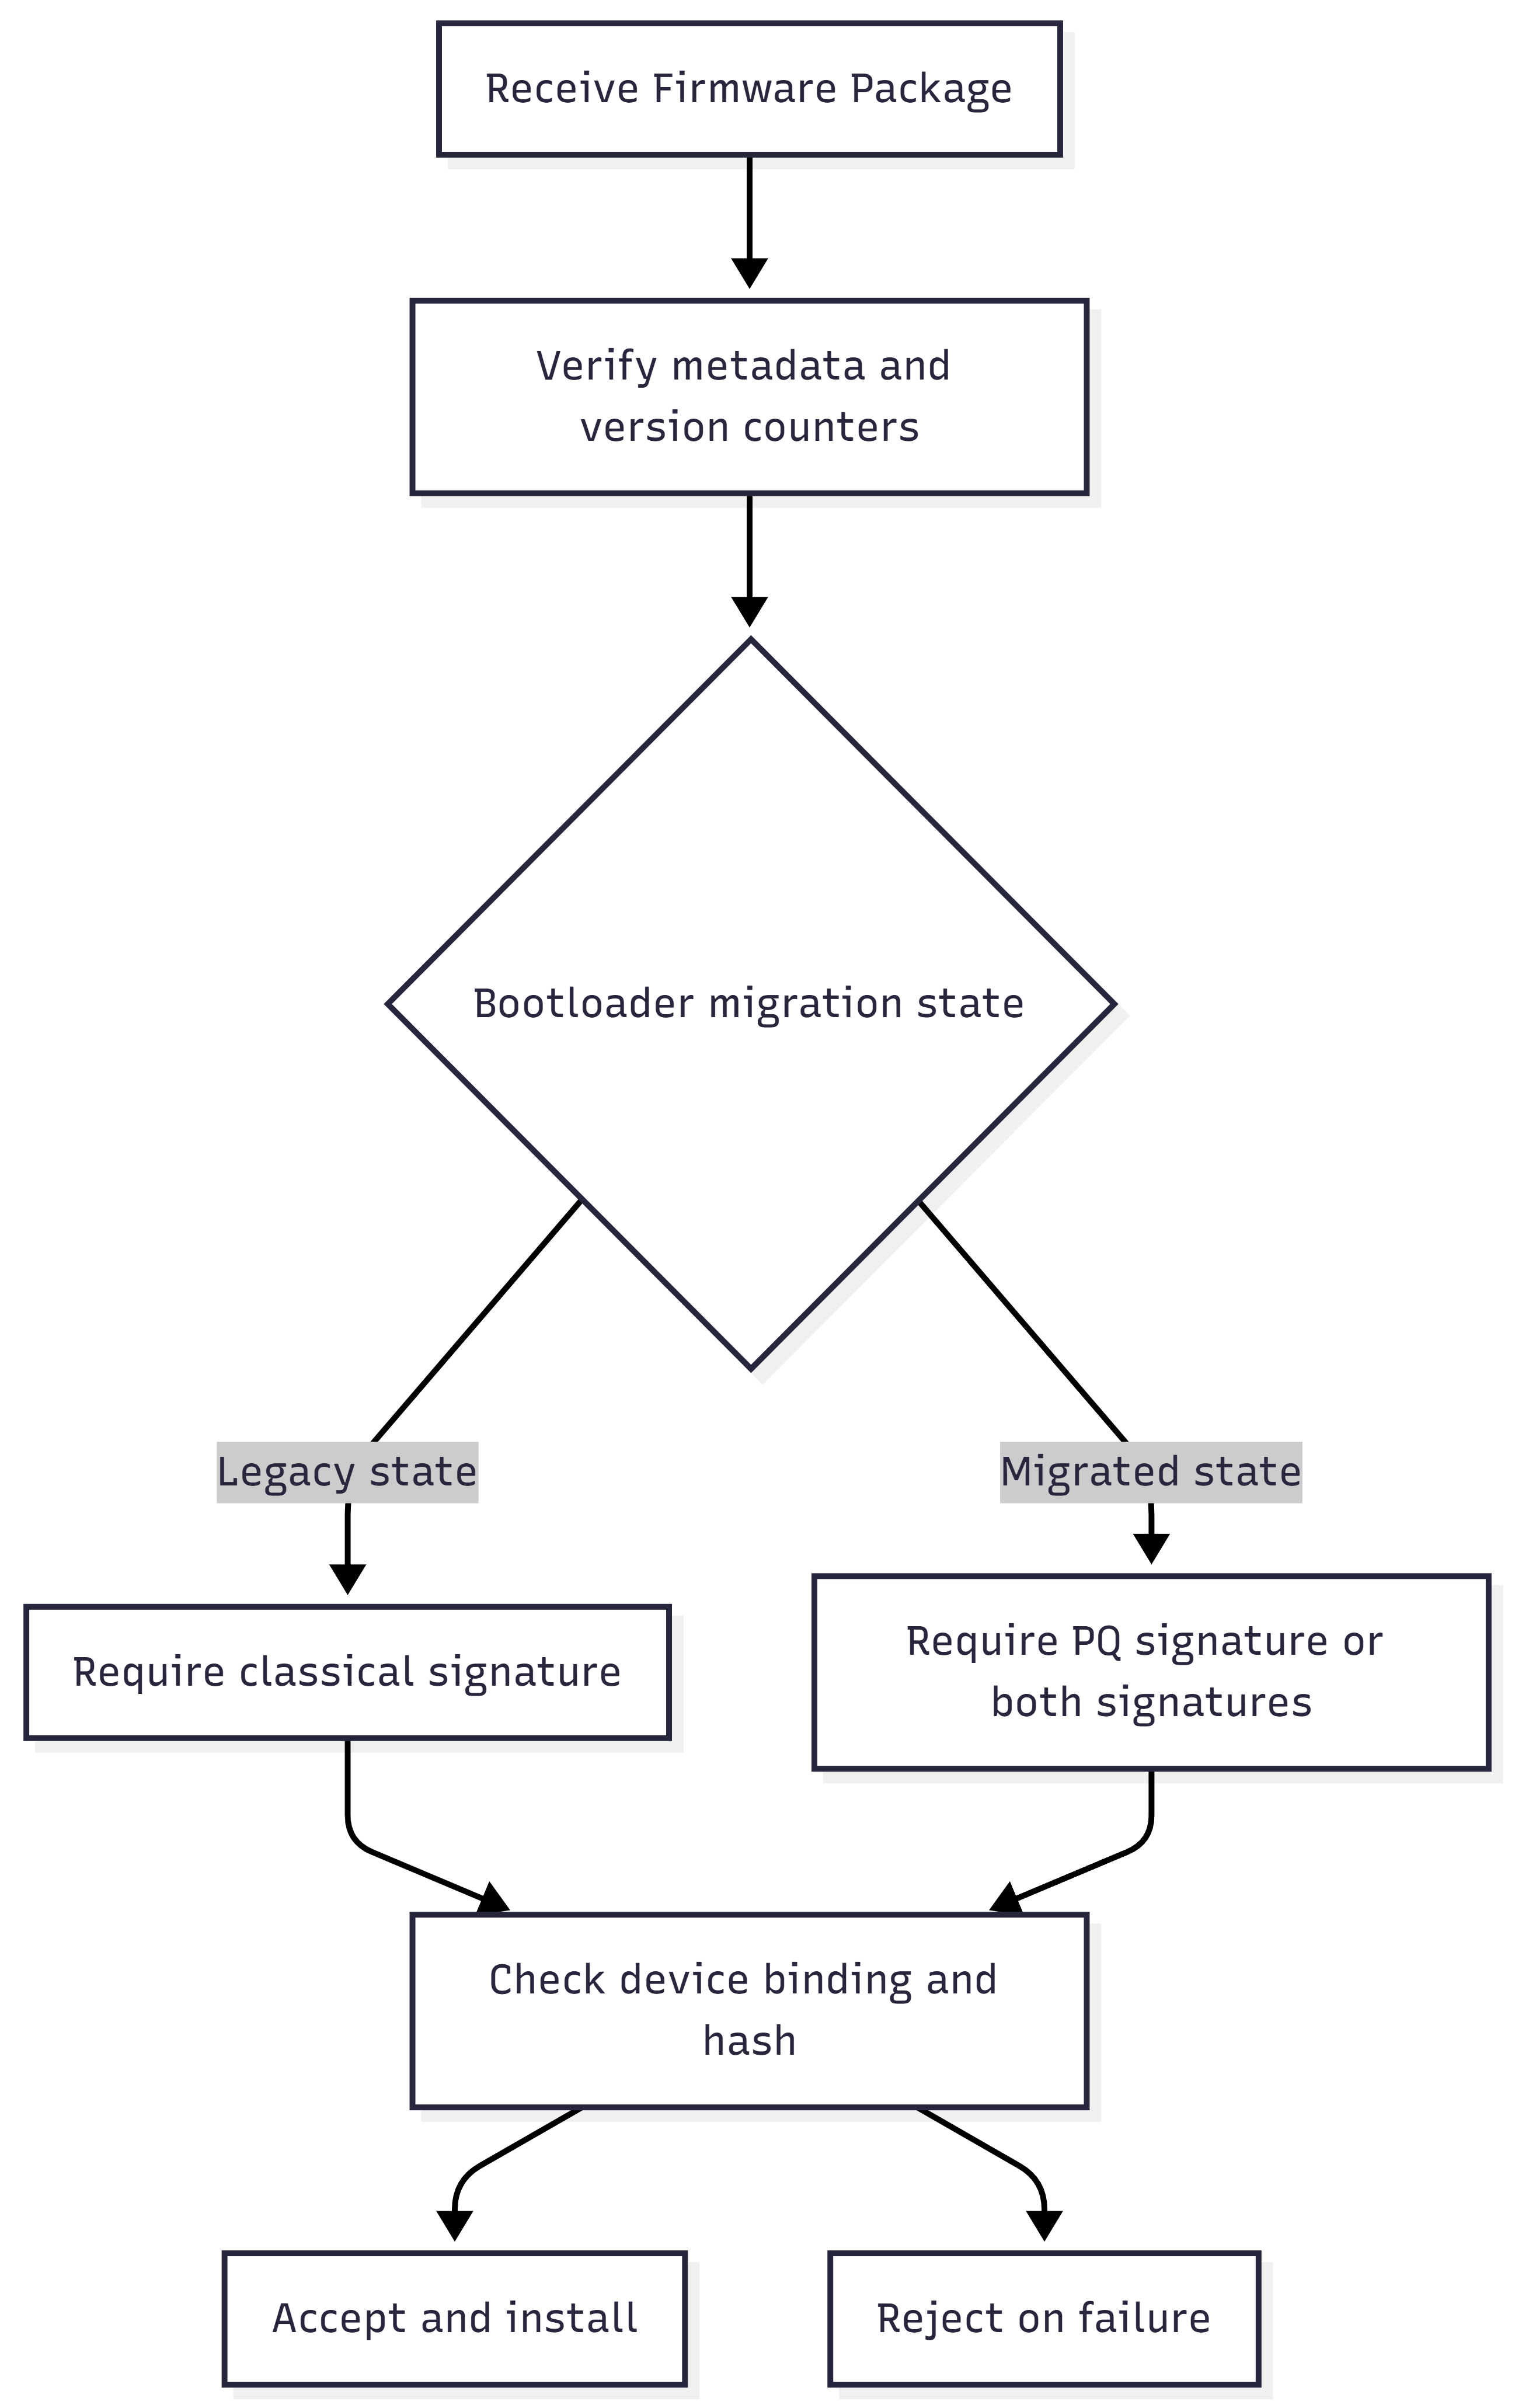
\includegraphics[width=0.9\columnwidth]{../images/policy.png}
\caption{Migration-policy flow for legacy and post-migration verification states.}
\label{fig:migration}
\end{figure}

\subsection{Limitations}

This study has two main limitations. First, it does not present cycle-accurate embedded benchmarks for ML-DSA or SLH-DSA on a specific microcontroller. Instead, it focuses on deployment-visible metrics that can be derived directly from the finalized standards and from policy logic. Second, the prototype treats signature validity abstractly; it models the presence of valid signatures rather than invoking a concrete PQC implementation.

These limitations are acceptable for the scope of this paper because the central claim is architectural: secure migration depends on authenticated metadata and downgrade-resistant policy, not only on choosing a larger or smaller signature. Future work can extend the prototype with real verifier benchmarks on an embedded platform and with certificate-chain modeling for production firmware ecosystems.

\section{Conclusion}

This paper evaluated the suitability of ML-DSA and SLH-DSA for post-quantum firmware signing and argued that the migration problem is broader than replacing ECDSA or RSA with a new primitive. Firmware trust depends on signed metadata, anti-rollback state, device binding, and verification policy, especially when classical and post-quantum signatures coexist during a transition period.

The standards-based comparison and prototype-driven evaluation show that ML-DSA is the most practical default for general firmware-signing deployments because it provides post-quantum security with substantially smaller signatures than SLH-DSA. SLH-DSA remains important as a conservative backup with different assumptions, but its large signatures can impose substantial overhead on small boot components. The policy simulation further showed that unrestricted either-valid verification leaves a downgrade path to classical-only signatures, whereas version-gated and both-required policies prevent that outcome.

Future work can add device-level benchmarks, real verifier implementations, certificate-chain handling, and measured secure-boot integration. Even without those extensions, the present results already show that a successful post-quantum firmware migration must combine cryptographic modernization with authenticated policy design.

\input{sections/acknowledgment}

\bibliographystyle{IEEEtran}
\bibliography{references}
\section*{Repository}

The implementation code, experimental scripts, and document source for this paper are publicly available at the following GitHub repository:

\begin{center}
\underline{\url{https://github.com/Nayekah/post-quantum-signing}}
\end{center}

\input{sections/statement}

\end{document}
